

	\documentclass[12pt,             % Schriftgroesse
               a4paper,          % Papierformat
               %liststotoc,      % (alt) Tabellen- und Abbildungsverzeichnis im Inhaltsverz.
               listof=totoc,     % Tabellen- und Abbildungsverzeichnis im Inhaltsverz.
               %idxtotoc,        % (alt) Index im Inhaltsverz. auffuehren
               index=totoc,      % Index im Inhaltsverz. auffuehren
               %bibtotoc,        % (alt) Literaturverzeichnis im Inhaltsverz. auffuehren
               bibliography=totoc,% Literaturverzeichnis im Inhaltsverz. auffuehren
               %oneside,         % auskommentieren, wenn beidseitig gedruckt wird
                                 % default ist 'twoside'
               BCOR1cm,          % zusaetzlicher Bindungsrand
               %english,ngerman   % TODO : Englisch als weitere Sprache, Deutsch als Hauptsprache
               ngerman,english  % TODO : alternativ Deutsch als weitere und Englisch als Hauptsprache
               ]{scrbook}

%%%%%%%%%%%%%%%%%%%%%%%%%%%%%%%%%%%%%%%%%%%%%%%%%%%%%
% Pakete einbinden (Reihenfolge ist z.T. wichtig!)
%%%%%%%%%%%%%%%%%%%%%%%%%%%%%%%%%%%%%%%%%%%%%%%%%%%%%
\usepackage[latin1]{inputenc}   % Eingabezeichenkodierung, alternativ "ansinew"
                                %  (Windows only) oder "utf8" fuer Unicode
\usepackage{cmap}               % Fuer schoene Ligaturen in PDFs
\usepackage[T1]{fontenc}        % u.a. Umlaute als ein Zeichen in der PDF-Datei
\usepackage{lmodern}            % Linux Modern Schriften auswaehlen
\usepackage{graphicx}           % Um Bilder einzubinden (mit \includegraphics)
\usepackage{subfigure}
\usepackage{tikz}               % Um Latex Grafiken zu erstellen
\usepackage{makeidx}            % Falls ein Index erstellt werden soll, muessen

\makeindex                      %  die beiden Zeilen aktiviert werden.
                                %  zusaetzlich noch \printindex unten
\usepackage{units}              % Einheiten setzen mit z.B. \unit[10]{MB} und \unitfrac[100]{Mbit}{s}
\usepackage{amsmath}
\usepackage{amsthm}
%\usepackage{siunitx}           % Wesentlich umfangreicheres Einheiten Paket als Ersatz fuer "units"
\usetikzlibrary{arrows,shapes}  % Fuer Latex Grafiken
\usetikzlibrary{calc}

% In dieser Datei koennen eigene Erweiterungen eingebracht werden
% HIER: Nur wenn noetig Datei my_includes.tex aendern
% Hier eigene Definitionen und zus�tzlich gebrauchte Pakete einbinden
         % Eigene Pakete und Definitionen laden

% letztes:     ----------------------------------------------------------------------------------------------------
\usepackage{hpcdasa}           % HPC-Vorlage fuer Bachelor-, Master- und Studienarbeiten 
                               %  mit Titelseite
% dieses sollte immer als letztes eingebunden werden, da es hyperref mitbringt 
% (welches wirklich das letzte ist)

%%%%%%%%%%%%%%%%%%%%%%%%%%%%%%%%%%%%%%%%%%%%%%%%%%%%%%%%%%%%%%%%%%%%%%%%%%%%%%%
% Hier beginnt das eigentliche Dokument
%%%%%%%%%%%%%%%%%%%%%%%%%%%%%%%%%%%%%%%%%%%%%%%%%%%%%%%%%%%%%%%%%%%%%%%%%%%%%%%
\begin{document}

%% Ein paar wichtige Details konfigurieren
%%----------------------------------------
% HIER: Details anpassen in my_config.tex
%
% my_config.tex
%
% Diese Datei dient dazu, die Vorlage anzupassen.
% TODO : alle Einstellungen anpassen.
%

% Ein paar Variablen f�r die Titelseite
\author{Liangkun He}                             % Name des Autors
\matnr{374300}                                       % Matrikel-Nummer
\reporttype{Bachelorarbeit}                          % Studienarbeit/Diplomarbeit/Bachelorarbeit/Masterarbeit
\titleDe{Ausf�hrliche Untersuchung der Speicherzugriffe: Erweitertes Roofline-Modell f�r Energieoptimierung}         % Deutscher Titel
\titleEn{A Deep Dive into Memory Access: Extended Roofline for Power Management}       % Englischer Titel
% bitte beide Titel eintragen.

%\addsupervisor{Prof.\,Dr.\,rer.\,nat. Matthias~S.~M\"{u}ller}       % Betreuer
%\addsupervisor{Prof. Dr. Matthias~S.~M\"{u}eller}      % weitere Betreuer (bei Bedarf)

% Falls es einen Zweitgutachter gibt
%\addsecondreferee{Univ.-Prof.\,Dr.\,rer.\,nat. Unbekannt} % Zweitgutachter

% Falls mehrere Institute die Arbeit betreuen
\addinstitute{hpc}{Lehrstuhl f\"{u}r Hochleistungsrechnen, RWTH Aachen University\\
IT Center, RWTH Aachen University}{(')}
\addinstitute{lfbs}{Lehrstuhl f\"{u}r Betriebssysteme, RWTH Aachen University}{(*)}
\addsupervisor[hpc]{Prof.\,Dr.\ Matthias~S.~M\"{u}ller}
%\addsupervisor[hpc]{Manni Mustermann}                               % Erstgutachter
\addsecondreferee[lfbs]{Prof.\ Dr.\ 	Martin Schulz}               % Zweitgutachter
\addadviser[hpc]{Bo Wang, M.Sc.}                               % Betreuer/ Assistent
               % TODO : bearbeite Einstellungen in my_config.tex

%%%%%%%%%%%%%%%%%%%%%%%%%%%%%%%%%%%%%%%%%%%%%%%%%%%%%
% Der Vorspann (andere Seitennummerierung)
%%%%%%%%%%%%%%%%%%%%%%%%%%%%%%%%%%%%%%%%%%%%%%%%%%%%%
\frontmatter

\maketitle                %Titelseite ausgeben
\cleardoublepage
\printversicherung        %Versicherung, dass Arbeit selbstaendig erstellt wurde


% TODO : die Abstracts sind optional.
% Falls Datei abstract.tex existiert, diese einbinden
\IfFileExists{abstract.tex}
	{\cleardoublepage\phantomsection\pdfbookmark{\abstractname}{abstract} %% fuegt ersten Abstract in die Bookmarks ein
	 \begin{otherlanguage}{ngerman}
\begin{abstract}
  Angesichts der gesteigerten Leistung von Supercomputern war der Stromverbrauch in den letzten Jahren von grosser Bedeutung. Laut der TOP-500-Liste reicht der Stromverbrauch der heutigen Top-10-Supercomputer von 1 MW bis 30 MW. Ein erheblicher Stromverbrauch kostet nicht nur viel Geld, sondern erhoeht auch den Kohlendioxidausstoss. Riesige HPC-Cluster erzeugen grosse Waermemengen, die gekuehlt werden muessen. Es ist wichtig, den Stromverbrauch zu reduzieren und gleichzeitig eine hohe Leistung fuer Supercomputer aufrechtzuerhalten.
  
  Supercomputer bestehen aus Rechenknoten. Jeder Knoten enthaelt Mikroprozessoren, Hauptspeicher, GPU und Festplatte. Der Mikroprozessor traegt einen grossen Teil zum Stromverbrauch bei, da er fuer die meisten Rechenaufgaben verantwortlich ist. Moderne Prozessoren bestehen aus Core und Uncore. Der Core hat Komponenten, die Anweisungen ausfuehren. Der Uncore verfuegt ueber nicht-rechenbezogene Funktionalitaeten, einschliesslich Datenuebertragung zwischen dem Prozessor und anderen Komponenten, Energieverwaltung und Kommunikation zwischen den Sockeln. Core und Uncore haben ihre eigenen Taktfrequenzen. Diese Arbeit untersuchte, wie sich die Uncore-Frequenz auf die Leistung und den Stromverbrauch auswirkt und untersuchte, wie die Leistungsengpaesse basierend auf dem Roofline-Modell zu charakterisieren sind. 
  
  Das traditionelle Roofline-Modell geht davon aus, dass sich die Kernausfuehrungen und die Datenuebertragung zwischen Prozessor und Speicher perfekt ueberlappen, aber in Wirklichkeit gibt es solche Situationen nicht immer. Einige Programme koennen unter Speicherlatenz leiden. Die Speicherlatenz ist die Zeit, in der der Prozessor eine Speicheranforderung initiiert, bis die Daten verfuegbar sind. Da der Prozessor viel schneller ist als der Speicher, wird er bei Speicherlatenz blockiert. Daher ueberschneiden sich Berechnung und Datenuebertragung nicht immer perfekt. Obwohl moderne Prozessoren ueber mehrere Techniken verfuegen, um die Speicherlatenz zu reduzieren, koennen sie die Latenz nicht vollstaendig eliminieren. Diese Arbeit schlaegt eine erweiterte Roofline-Methode vor, die das Roofline-Modell mit Zeitintervallanalyse kombiniert, um die Speicherlatenz zu erkennen und ihre Auswirkungen auf die Leistung zu analysieren. Die erweiterte Roofline-Methode ist in einen Algorithmus integriert, der die Leistung durch dynamisches Modifizieren der Core- und Uncore-Frequenzen des Prozessors optimiert. Die experimentellen Ergebnisse zeigen, dass das Verfahren eine Energieeinsparung von bis zu 9,4\% bei einer Verlangsamung im schlimmsten Fall von 6,5\% erreicht. Das Verfahren erreicht auch im besten Fall 6,2\% Beschleunigung und 8,9\% Energieeinsparung gegenueber der Standardeinstellung bei gleicher Leistungsbegrenzung. 
  
  \bigskip\par
  \textbf{Stichw"orter:} Roofline Modell,  Speicher Latenz,  Energieverwaltung,  Leistungsoptimierung 
\end{abstract}
\end{otherlanguage}
\begin{otherlanguage}{english}
\begin{abstract}
	With the increased performance of supercomputers, power consumption has been of great concern for recent years. According to the TOP 500 list, the power consumption of today's top 10 supercomputers ranges from 1 MW to 30 MW. Significant power consumption costs not only a vast sum of money but also raises carbon dioxide emissions. Huge HPC clusters generate great amount of heat that requires cooling. It is important to reduce power consumption while maintaining high performance for supercomputers. 
	
	 Supercomputers consist of computing nodes. Each node contains microprocessors, memory, GPU and storage. The microprocessor contributes a large portion of power consumption because it is responsible for most computational tasks. Modern processors consist of core and uncore. The core has components that execute instructions. The uncore has non-compute-related functionalities including data transfer between the processor and other components, power management and inter-socket communications. The core and uncore have their own clock frequencies. This work explored how the uncore frequency affects the performance and power consumption and studied how to characterise the performance bottlenecks based on the Roofline model. 
	 
	 The traditional Roofline model assumes the core executions and data transfer between the processor and memory overlap perfectly but in reality, such situations do not always exist. Some applications may suffer from memory latency. The memory latency is the time when the processor initiates a memory request until the data is available. Since the processor is much faster than memory, it stalls when there exists memory latency. Therefore, the computation and data transfer do not always overlap perfectly. Though modern processors have several techniques to reduce the memory latency, they cannot eliminate the latency completely. This work proposes an extended Roofline method that combines the Roofline model with time interval analysis to detect the memory latency and analyse its impact on performance. The extended Roofline method is integrated with an algorithm that optimizes the performance by dynamically modifying the core and uncore frequencies of the processor. The experimental results show that the method achieves up to 9.4\% energy saving with the worst-case slowdown of 6.5\%. The method also achieves in best case 6.2\% speedup and 8.9\% energy saving compared to the default setting under the same power cap.
	 
  \textbf{Keywords:} Roofline model,  Memory Latency, Power management, Performance optimization
\end{abstract}
\end{otherlanguage}

	}{}


\cleardoublepage
\phantomsection\pdfbookmark{\contentsname}{toc}
\tableofcontents          %Inhaltsverzeichnis

\listoffigures            %Abbildungsverzeichnis

\listoftables             %Tabellenverzeichnis

%%%%%%%%%%%%%%%%%%%%%%%%%%%%%%%%%%%%%%%%%%%%%%%%%%%%%
% Der Hauptteil ("normale" Seitennummerierung)
%%%%%%%%%%%%%%%%%%%%%%%%%%%%%%%%%%%%%%%%%%%%%%%%%%%%%
\mainmatter
% Hier werden die Kapitel eingebunden
% TODO : weitere Kapitel in my_chapters.tex eintragen
% Hier die Kapitel des Hauptteils einf�gen
\chapter{Introduction}

For decades,  high-performance-computing systems have become faster than ever thanks to the powerful multi-core microprocessors. While processors deliver a significant amount of floating-point operations per second, power consumption becomes a major challenge. Fugaku, the world's top supercomputer, consumes 29.89MW to deliver 442 PFlop/s \cite{1}. Consequentially, the energy cost under such power consumption is significant, e.g. 29MW at \$0.12/kWh \cite{26} is \$3480 an hour about over \$30 million per year. Moreover, massive carbon dioxide emissions are noticeable, more manpower is needed to maintain them. As a result, people decided to set power budgets on high-performance computers and scientists tried numerous methods to find the balance between high performance and energy efficiency. For example, the Department of Energy (DOE) of the U.S has set a power budget of 30 MW on one of the exascale computing systems Frontier that yet to come \cite{2}. To achieve such a goal, it is important to find a reliable power management approach.

Supercomputers consist of large amounts of computing nodes. Each node is just like a computer or laptop people daily use except it is more powerful in terms of the computing speed of the processor, memory capacity and GPU. The power consumption mainly comes from those components. The microprocessor is the kernel of a supercomputer. It consists of two components namely core and uncore. In short, the core is responsible for computational works while uncore for non-compute-related works such as data transfer. Each of the components has its own frequency.  Running average power limit (RAPL) is a feature of Intel processors to set power caps to ensure the CPU and memory do not exceed the power budget \cite{3}.  However, RAPL does not aware of whether the application is compute-intensive or memory-intensive. As a result, RAPL may reduce the uncore frequency though the running program is memory bounded, e.g. STREAM benchmark that heavily demands the uncore resources. 

The Roofline model estimates the performance of an application based on its operational intensity. It can distinguish whether an application is memory- or compute-bound. However, the Roofline model assumes perfect overlap between computation and data transfer. In reality, such a case does not always exist because some applications suffer from high memory access latency. It is important to detect the memory latency and analyse how it affects performance.

In this paper, I propose to extend the Roofline model with a method \textit{time interval analysis}, which detects the memory access latency in the runtime and analyses its impact. Then the core and uncore frequency will be modified accordingly to achieve power saving. The method is implemented with the sampling approach, which means it initiates an interrupt after a certain time frame, analyses hardware activities of the time interval and optimizes the performance by modifying the components' frequency. The paper makes the following contributions:
\begin{enumerate}
\item Introduce the hardware architecture of the modern high-performance computers.
\item Analyse the uncore frequency scaling and its impact on performance, power consumption.
\item Extend the Roofline model with time interval analysis. It is able to detect memory latency and reduce the power consumption during runtime. 
\item Evaluate the extended Roofline method with multiple HPC benchmarks on a node to show the power and energy saving.
\end{enumerate}

The remainder of the paper is organized as follows. Section 2 provides scientific backgrounds. Section 3 describes the Roofline model and propose the time interval analysis. Section 4 shows the implementation. Section 5 discusses the experimental results. Section 6 contains related work. Section 7 summarises the work and draws conclusions.

\chapter{Overview and Background}

\section{Hardware Architecture}

Supercomputers are usually designed with the cluster architecture that consists of a set of computing nodes. In the great majority of cases, all nodes use the same hardware and the same operating system. The nodes are connected via fast interconnect to accomplish great task parallelism. Users log on to the head node via ssh. They can distribute several tasks on computing nodes. A node may look similar to any other personal computer but is far more powerful in terms of computing power.  The nodes also have access to global data storage.

\begin{figure}[htbp]
\centering
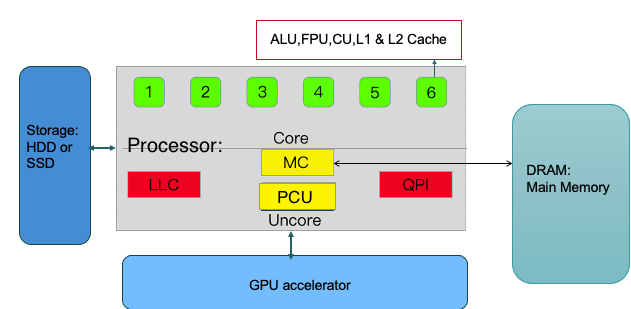
\includegraphics[width=11cm]{pictures/fig2.2}
\caption{Node}
\end{figure}

Figure 2.1 represents a computing node. It consists of processors, DRAM, local storage, and GPU accelerators. Today's microprocessors are mainly based on von Neumann architecture. The processor is divided into two areas namely core and uncore. The core consists of components that are responsible for computing and executing instructions, including control units (CU), arithmetic logic units (ALU), floating point unit (FPU),  and upper-level caches e.g. L1 and L2 cache.  The uncore contains other components that are not responsible for the computational tasks but must be closely connected to the core such as the last level cache (LLC), the memory controller (MC), the quick path interconnect (QPI) and the power control logic (PCU).  They are responsible for data communication between the processor and other components, power setting of the processor and inter-socket communication. When a program utilises core heavily, it is called compute-intensive. Instead, if a program is memory-intensive, high uncore activities will be observed. 

\subsubsection{Core}
Moore's law suggests that the number of transistors in a dense  integrated circuit doubles every one to two years \cite{39}. As a result, the clock frequency of microprocessors has grown exponentially over the last century. However, high clock frequency brings significant power consumption. Electric power brings heat dissipation problems. That is the reason that the growth rate of the clock frequency of a single core has decreased for the last few decades. If the clock frequency is too high, the cooling system of the processor cannot dissipate heat fast enough that it may damage the hardware. 

To increase the performance of the processor and limit the heat problems simultaneously, people start to focus on the development of multi-core processors. The processor showed in figure 2.1 is a 6-core processor. Each core has its own ALU, FPU, L1, and L2 cache.  Multi-core processors have huge advantages on task parallelism over single-core processors. For example, multi-core processors can break a huge task into small pieces and assign each piece to a core. Each core can operate at a lower frequency and therefore costs lower energy.
\subsubsection{Uncore}
As the core count and the size of LLC increases, the uncore occupies more on die-area \cite{17}, which contributes significant power consumption \cite{18} to the processor. The function of uncore is managing non-compute intensive workloads such as data communication between the processor and other components. The LLC is a fast but small memory located in uncore area. It stores a small amount of data that are likely to be used by the core since the core accesses the LLC much faster than the DRAM. The MC is responsible for the data communication with DRAM. The QPI allows the multiple-socket platform to communicate between sockets \cite{17}. The PCU modifies clock frequency and core voltage to coordinates the power and performance ratio \cite{17}.
\subsubsection{Memory Hierarchy}
For the last few decades, the semiconductor industry has divided microprocessors and memory into two different fields. The technology for microprocessors focused on speed while for memory on capacity. As a result, the performance improvement rate of microprocessor speed outpaced the improvement rate of memory speed \cite{10}. Figure 2.2 \cite{9} showed that the performance gap between processor and memory has been growing for the last few decades.

\begin{figure} [h] %hier können noch Positionierungswünsche angegeben werden
	\centering   % Alles weitere zentrieren
	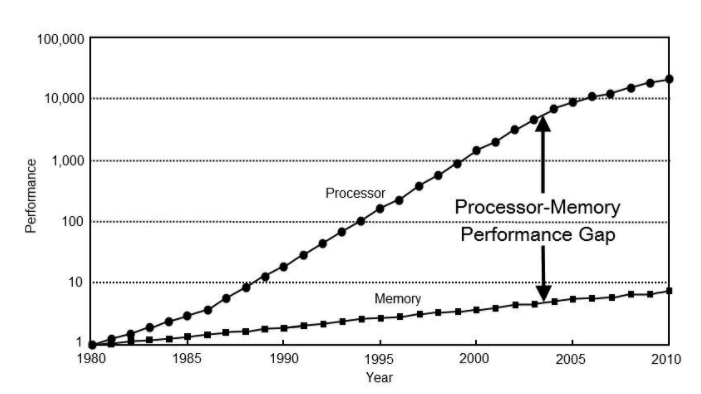
\includegraphics[width=10cm]{pictures/fig2.4}
	\caption{Performance gap between processor and memory \cite{9}}
	\label{fig1}  %Reihenfolge ist wichtig! Immer erst \caption{} dann \label{}
\end{figure}

When the processor encounters memory-intensive programs, the continuous access to the memory makes the processor wait for slower memory and stall, therefore it wastes a lot of clock cycles. In order to solve the performance gap issue, the cache is introduced. The cache is implemented as smaller size but fast accessing speed SRAM memory which located inside the processor. It is further divided into several levels. For example, Intel's processors usually have L1, L2, and L3 cache. The L1 and L2 cache are inside the core while the L3 cache is located in uncore area. The CPU is connected to different levels of memory. Figure 2.3 \cite{11} shows the abstract of the memory hierarchy. The closer the memory to the CPU, the faster but smaller it will be. When a CPU requires data, it first accesses the register directly and then followed by the cache. If the data item is not in the cache, then there is a cache miss and the processor will continue searching the main memory until the data item is found.			
	
\begin{figure} [h] %hier können noch Positionierungswünsche angegeben werden
	\centering   % Alles weitere zentrieren
	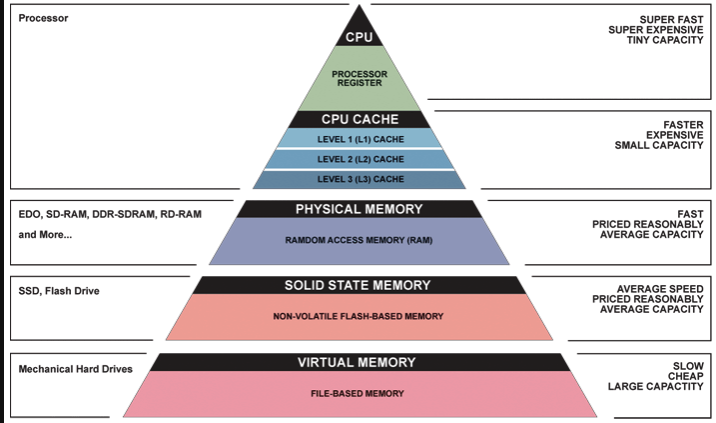
\includegraphics[width=10cm]{pictures/fig2.5}
	\caption{Memory hierarchy \cite{11}}
	\label{fig1}  %Reihenfolge ist wichtig! Immer erst \caption{} dann \label{}
\end{figure}

\subsubsection{Graphic Processing Unit}
A GPU is a specialized processor to accelerate graphics rendering. The biggest difference between a GPU and a CPU is that the GPU has thousands of sub-cores. This makes the GPU more efficient than the CPU on parallel computing. Today's supercomputers commonly use a general purpose graphics processing unit (GPGPU) which not only handles computation for computer graphics but also performance general CPU tasks. In some applications that require massive vector operations, the GPGPU is proven to be far more efficient than the CPU. In this work, the focus is on the tuning of the processor's frequency.

\section{Power Management}
The thermal design power (TDP) is the maximum power that the cooling system in a computer is needed to dissipate. It is not the maximum power a processor can consume but a power budget for the system to operate safely. For example, a processor is designed with 50W TDP, which means that the cooling system can dissipate in maximal 50W of heat without exceeding the maximum temperature for the CPU. HPCs have several functionalities to maintain a power consumption and make sure it operates safely.
\subsubsection{Running Average Power Limit}
Running Average Power Limit (RAPL) is a mechanism implemented in hardware that monitors the power consumption of CPU and DRAM \cite{19}. It was first introduced in Intel's Sandy Bridge microarchitecture. RAPL provides several counters to monitor the power and energy consumption of the processor package and DRAM over a sliding time frame. Another functionality of RAPL is to maintain a power cap of the average power consumption of the processor. Programmers can measure or constrain the power consumption of DRAM and processor package(core and uncore) by modifying the model-specific registers (MSRs) \cite{21}.
\subsubsection{Dynamic Voltage and Frequency Scaling}
DVFS \cite{22} is a widely used technique to save power on modern computers. According to Etienne Le Sueur et al., the dynamic power consumption is 
\begin{equation}
P = CfV^2
\end{equation}
where $P$ is the dynamic power, C is the capacitance and V is the voltage. When the frequency is lowered, the corresponding voltage will be reduced significantly. DVFS dynamically modifies the core frequency and the supply voltage to achieve power saving.

%\subsubsection{LIKWID}
%LIKWID is short for "like I know what I'm doing".
\subsubsection{Uncore Frequency Scaling}
Intel separates the core and uncore frequency from the Haswell microarchitecture onward. The uncore frequency scaling (UFS) is therefore introduced. Programmers can use UFS to modify the uncore frequency regardless of the core's operating state \cite{21}. This subsection analyses the impact of uncore frequency on performance using one Haswell node. The node contains one Intel(R) Xeon(R) processor E5 v3 @ 2.30GHz which has 18 cores. The node has 32GB of memory. 

Three benchmarks from the NAS parallel benchmark \cite{23} suit namely Block Tridiagonal solver (BT), Multi-grid solver (MG) and Embarrassingly Parallel (EP) are used. BT is an LLC cache-bound benchmark, MG is a memory-bound benchmark and EP is a compute-intensive benchmark. Each of them has unique performance characteristics that help to evaluate the impact of uncore frequency on performance. The openMP version of those benchmarks are  used. The uncore frequency is reduced from 3.0 GHz to 1.2 GHz in steps of 0.1 GHz. The PKG power and DRAM power in Watts,  completion time in seconds and memory bandwidth in GB/s are recorded. The experiments were repeated 3 times and the average values of the result  are presented. 

Table 2.1 presents the completion time, PKG power, DRAM power, memory bandwidth and last level cache miss per second for BT, MG and EP at default uncore frequency (3.0GHz). All of them are measured by LIKWID. Figure 2.4 (a), (b) and (c) present the performance impact of uncore frequency on those data. The x-axis is the uncore frequency while the y-axis shows all the data normalised with respect to the default uncore frequency (3.0 GHz). 

\begin{table} %[htbp] %hier können noch Positionierungswünsche angegeben werden
	\centering      % Alles weitere zentrieren
	\begin{tabular}{|c|c|c|c|} %Alle Spalten zentrieren, ansonsten 'r' oder 'l'
		\hline
		\textbf{Metric} & \textbf{BT} &\textbf{MG} & \textbf{EP}  \\
		\hline
		Completion time(s)              & 75.4  & 1.2  &    5.56        \\
		\hline
		PKG power(W)	              &  140& 119 &   129.      \\
		\hline
		DRAM power(W)		 &   11 &   16 & 5 \\
		\hline	
		Memory bandwidth(GB/s)  &  20 & 41 & 0.049\\

		\hline

		
		
		\hline
	\end{tabular}
	\caption{Performance metrics for BT, MG and EP @ 3.0 GHz}
	%\label{tab:vergleich}  %Reihenfolge ist wichtig! Immer erst \caption{} dann \label{}
\end{table}

Figure 2.4 (a) presents the performance impact of uncore frequency on the memory-bound benchmark MG. As the uncore frequency is reduced from 3 GHz to 1.4 GHz, the job completion time increases linearly. When the uncore frequency is lowered under 1.4 GHz, the completion time increases faster. It suggests that for memory-bound applications, the decrease in uncore frequency results in significant performance degradation. The reason is that the memory controllers operate slower at a lower uncore frequency \cite{21}. There will be fewer memory requests that are sent by the controllers. Therefore, the DRAM power decreases which makes the DRAM read or write data slower. 

Figure 2.4 (b) presents the results on the compute-bound benchmark EP. As the uncore frequency is reduced, the PKG power decreases significantly. In the meantime, the job completion time is not affected. There are no obvious changes on the DRAM power and memory bandwidth because EP does not utilize memory controller nor LLC\cite{21}. For compute-bound applications, the uncore frequency can be reduced to achieve power-saving without performance downgrading.

Figure 2.4 (c) presents the results on the LLC-bound benchmark BT. The DRAM power does not change during the experiment. When the uncore frequency is greater than 2.5 GHz, there are no obvious changes on each of the datasets.  As the uncore frequency is reduced from 2.5 GHz to 1.7 GHz, the package power and memory bandwidth decrease but the execution time increases slowly. When the uncore frequency is reduced under 1.7 GHz, the completion time increased aggressively. For LLC-bound applications, it is possible to reduce the uncore frequency within a certain limit. If a small-scale of performance downgrading is acceptable, the uncore frequency can be reduced sightly to save power.

From the result of Figure 2.4, the following conclusions can be drawn
\begin{enumerate}
\item Lowering the uncore frequency downgrades the memory-intensive applications
\item For compute-intensive applications the uncore frequency can be lowered without performance downgrading.
\item For LLC intensive applications the uncore frequency can be lowered up to a certain limit.
\end{enumerate}

\begin{figure}
  \centering
  \subfigure[MG]{
    \label{fig:subfig:a} %% label for first subfigure
    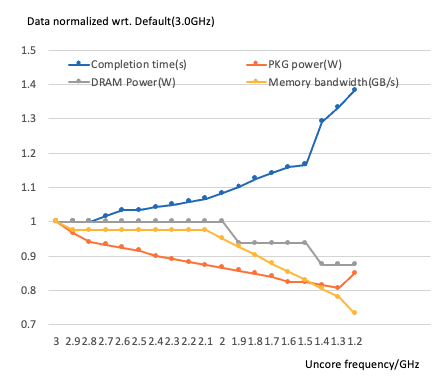
\includegraphics[width=3in]{pictures/mg}}
  \hspace{0.000001in}
  \subfigure[EP]{
    \label{fig:subfig:b} %% label for second subfigure
    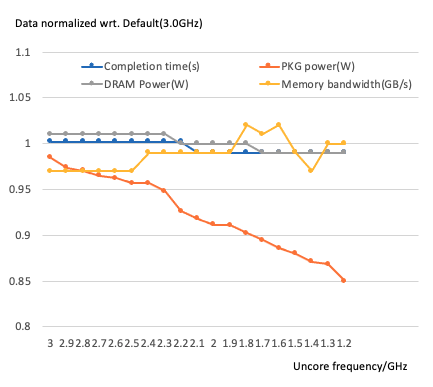
\includegraphics[width=3in]{pictures/ep}}
     \hspace{0.000001in}
  \subfigure[BT]{
    \label{fig:subfig:b} %% label for second subfigure
    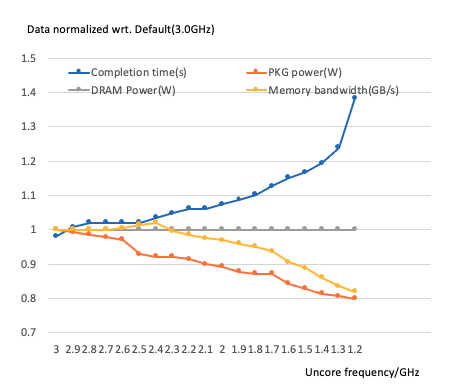
\includegraphics[width=3in]{pictures/bt}}
  \caption{Performance impact of uncore frequency on MG, EP and BT}
  \label{fig:subfig} %% label for entire figure
\end{figure}



\chapter{The Extended Roofline Model}
\section{The Conventional Rooflne Model}

The Roofline model estimates the performance of an application running on a multi-core processor by exploring the hardware limitations. The performance bottlenecks are characterised as computation and data transfer. Assuming a scenario that there are $B$ Gbytes of data transfer from the memory to the CPU. The processor has the peak performance of $P_{max}$ GFlops/s. The memory provides the maximal bandwidth of $BW$ GB/s. Assuming the processor finished $F$ floating-point operations and there is perfect overlap between computation and data transfer, the data transfer time is $B/BW$ seconds, and the processor takes $F/P_{max}$ seconds to finish all the operations \cite{12}. The total execution time is 
\begin{equation}
T = \max \begin{cases}
{F/(P_{max})}\\
{B/BW}
\end{cases}
\end{equation}
Since the performance is measured as GFlops/s, both sides of the equation can be divided by $F$ and the result is reciprocated. The attainable performance is hereby 
\begin{equation}
P = min\begin{cases}
{P_{max}}\\
{I*BW}
\end{cases}
\end{equation}

The peak performance of the processor and the peak memory bandwidth are hardware-specific given by the vendor. The realistic maximal memory bandwidth can be measured by the STREAM benchmark \cite{12}. The attainable performance is visualised as a function $P$ with one variable  $I = F/BW$. $I$ is defined as the arithmetic intensity or operational intensity. 

\begin{figure} [h] %hier können noch Positionierungswünsche angegeben werden
	\centering   % Alles weitere zentrieren
	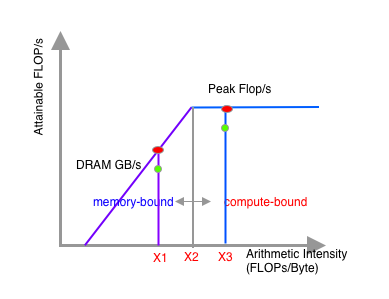
\includegraphics[width=9cm]{pictures/fig3.2}
	\caption{The Roofline model}
	\label{fig3.2}  %Reihenfolge ist wichtig! Immer erst \caption{} dann \label{}
\end{figure}

Figure 3.1 illustrates the Roofline the attainable performance depending on the arithmetic intensity. The x-axis is the arithmetic intensity and the y-axis is the attainable peak performance with logarithmic scales. The arithmetic intensity describes how many operations a kernel takes per data transfer. To determine whether an application is compute-bound or memory-bound, one simply compares the arithmetic intensity with the machine balance, which is the ratio of the peak performance to the peak bandwidth $P_{max}/Bandwidth$. The machine balance is hardware specific.

The arithmetic intensity $X_1$ is less than the machine balance $X_2$, which implies that the kernel spends more time on data transfer than computation. Therefore, the application is memory-bound. Its maximal attainable performance is $X_1 * BW$, which sits on the bandwidth ceiling (red dot for $X_1$). For some applications, the measured memory bandwidth does not necessarily reach the maximum, in this case, the actual performance is below the ceiling (the green dot for $X_1$). 

The arithmetic intensity $X_3$ is greater than the machine balance $X_2$, as a result, it is compute-bound. The attainable performance is $P_{max}$, which sits on the computational ceiling (red dot for $X_2$). In reality, the processors do not always attain the peak FLOP/s. For this case, it is represented by the green dot for $X_3$, which is below the computational ceiling.

\section{The Hierarchical Roofline Model}
%\begin{figure} [h] %hier können noch Positionierungswünsche angegeben werden
%	\centering   % Alles weitere zentrieren
%	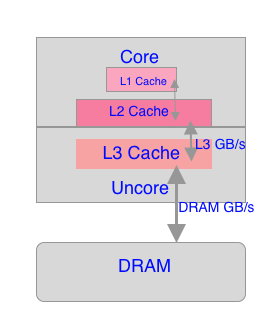
\includegraphics[width=4cm]{pictures/fig3.3}
%	\caption{Memory hierarchy}
%	\label{fig3.3}  %Reihenfolge ist wichtig! Immer erst \caption{} dann \label{}
%\end{figure}

Chapter 3.1 introduces the naive performance analysis on the kernel and DRAM. In reality, the Roofline model must be implemented on the hierarchical memory architecture, which is introduced in Chapter 2.1. In hierarchical memory architecture, different levels of memory have their individual bandwidths. As a result, each level has different machine balances. The data movement is also different for each level because applications have locality in a memory level. Therefore, it is important to construct the Roofline model for each memory level. This work focuses on the L3 cache and DRAM because their performances are affected by the uncore frequency. The L1 and L2 caches are located in the core area and their performances are affected by the core frequency. Two arithmetic intensities are calculated, one is the arithmetic intensity of the L3 cache, which is based on the data transfer between core and L3 cache; the other is the arithmetic intensity of DRAM, which is based on the data transfer between the processor and DRAM. 


\subsubsection{Bandwidth Ceilings}

Figure 3.2 (a) shows the Roofline function with two memory levels namely L3 cache and DRAM. The red line and the purple line represent the bandwidth ceilings for the L3 cache and DRAM respectively. Since the maximal L3 bandwidth is much higher than the DRAM. The machine balance of the L3 cache is smaller than DRAM. Assuming an application has the same measured intensities for both L3 and DRAM, the maximal attainable performance of L3 is higher than the DRAM's. As a result, the bandwidth ceiling of the L3 cache is always above the one of DRAM. 

In the hierarchical Roofline model, there exist several different arithmetic intensities. This indicates the performance bounds may be different for each memory level. In Figure 3.2 (a), the arithmetic intensity of the L3 cache $I_1$ is greater than the machine balance while the arithmetic intensity of DRAM $I_2$ is less than the machine balance. In this case, the performance is the minimum of those bound. This means it is bound to the minimal attainable FLOP/s. Since  $I_2 * BW_{DRAM}<I_1 * BW_{L3}$, the application is bound to DRAM.

\begin{figure}
  \centering
  \subfigure[L3 vs. DRAM]{
    \label{fig:subfig:a} %% label for first subfigure
    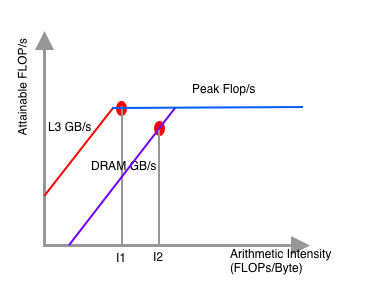
\includegraphics[width=2.9in]{pictures/fig3.4.png}}
  \hspace{0.000001in}
  \subfigure[Without SIMD or ILP]{
    \label{fig:subfig:b} %% label for second subfigure
    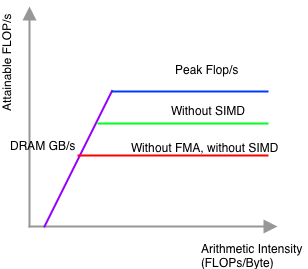
\includegraphics[width=2.5in]{pictures/fig3.5.png}}
  \caption{The hierarchical Roofline model}
  \label{fig:subfig} %% label for entire figure
\end{figure}

%In other word, the application is memory-intensive if one of the arithmetic intensities suggests memory bound, it is compute-intensive if both of the arithmetic intensities suggest compute bound. In figure 3.4 since $I_2 * bandwidth_{DRAM}<I_1 * bandwidth_{L3}$, the application is bound to memory.
\subsubsection{Computational Ceilings}
The peak Flop/s in Figure 3.2 (b) represents the theoretical upper bound of performance. In reality, applications do not always perform that well. There are several factors that affect the performance such as Single Instruction Multiple Data and Fused Multiply-Add instruction set when it comes to compute-bound situations. Those performance hindrances are mapped to the computational ceilings in Figure 3.2 (b).

\textit{Single Instruction Multiple Data (SIMD)}\\
SIMD is a method that allows a single instruction to process multiple data. SIMD has significant advantages against scalar operations on the array or vector data. Figure 3.4 presents the difference between SIMD and scalar operations. SIMD only needs one add instruction to operate the array addition. The scalar operation takes four add instructions to finish the task. Therefore, applications that utilize SIMD performs better than those that do not use SIMD. Therefore, in FIgure 3.2 (b), the computational ceiling of the applications that do not utilize SIMD is below the peak ceiling.

\begin{figure} [h] %hier können noch Positionierungswünsche angegeben werden
	\centering   % Alles weitere zentrieren
	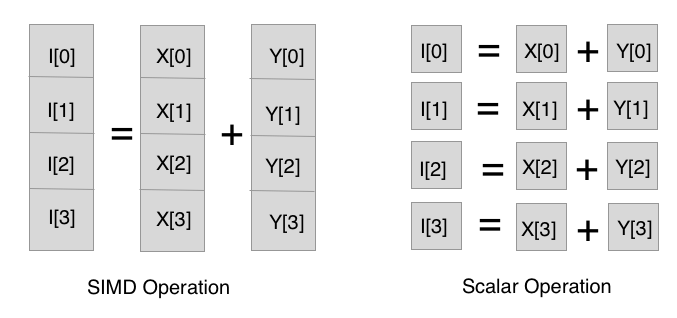
\includegraphics[width=10cm]{pictures/SIMD}
	\caption{Comparison of SIMD and Scalar Operation}
	%\label{fig3.1}  %Reihenfolge ist wichtig! Immer erst \caption{} dann \label{}
\end{figure}

\textit{Fused Multiply-Add (FMA)}\\
FMA is a technique that performs 2 floating-point operations (add and multiply) in one cycle. For example, FMA calculates an entire expression $X + (Y*Z)$ and rounds the final result to $N$ significant bits.  However, an unfused multiply-add would calculate $Y*Z$ and round it to $N$ significant bits. Then it adds the result to $X$ and round it to $N$ significant bits. 

For programs that calculate matrix multiplications, the adds and multiplies are often balance. However, some applications that solve PDEs on structured grids may be dominated by adds with very few multiplies \cite{12}. Those applications do not utilise FMA well. Their attainable performances are worse than those who are entirely dominated by FMA \cite{12}. Therefore, the red line in Figure 3.2(b) represents the computational ceiling for applications that do not utilise FMA. It is below the peak ceiling.\\
In conclusion, applications that do not utilise FMA or SIMD performs worse than others and have lower computational ceilings and smaller machine balances compared to others. 


\section{Time Interval Analysis}

\subsection{Memory Latency}
The memory latency is the delay between the CPU initiates a request until the data is received by the CPU. When the memory controller sends a request for a chunk of data, the upper-level cache L1 is first searched, if a cache miss occurs,  the processor continues to search lower level caches and finally the DRAM. The DRAM then sends the data to the CPU. The Roofline model assumes that there is perfect overlaps of the data transfer and computation because modern processors have several methods to reduce memory latency such as Out-of-Order execution and prefetching. 


\textit{Out-of-Order Execution (OoOE)}\\
In OoOE processor, instructions are stored into a buffer after being fetched and decoded \cite{13}. When the resources and execution units are available, the instruction will be assigned to the unit and then executed. The instructions do not have to be executed in a sequential manner any longer since they can leave the buffer before the older instructions. 

Modern processors operate many times faster than memory. Therefore, in an in-order execution processor, it costs several cycles in a pipeline stage to wait for the data to arrive. The processor has to stall and thus wastes all those cycles. OoOE processors, on the other hand, utilise those cycles to execute other instructions. As a result, it reduces the stalling time of the CPU. 

\begin{figure} [h] %hier können noch Positionierungswünsche angegeben werden
	\centering   % Alles weitere zentrieren
	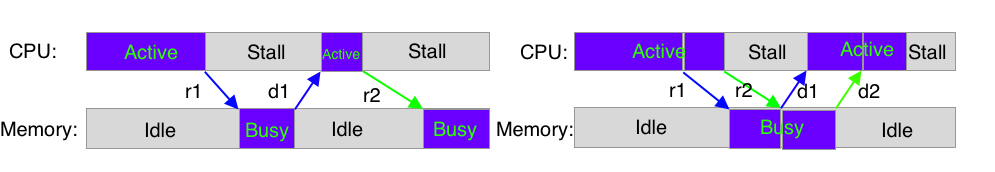
\includegraphics[width=15cm]{pictures/fig3.6}
	\caption{Comparison of in-order execution and OoOE}
	\label{fig3.5}  %Reihenfolge ist wichtig! Immer erst \caption{} dann \label{}
\end{figure}

Figure 3.4 illustrates the processor and memory activities during runtime. The figure on the left side shows the in-order execution. Assuming that we observe the activities in a certain time interval, the processor is proceeding with tasks at the beginning while the memory is idling because there are not any data requests. The processor then sends a data request $r1$ to the memory and begins to stall. The memory starts to read the data. Then it sends the data to the processor ($d1$) and returns to the idle state afterwards. The processor begins to proceed with the instruction. After the instruction is finished, the processor fetches and decodes the next one and then sends another data request $r2$. In this case, there are no overlaps between processor and memory. Therefore, the Roofline model cannot be applied here.

The figure on the right side shows the activities of the OoOE processor and memory. The only difference is that after sending the first data request $r1$, the processor searches the instruction queue to find an instruction whose resources and functional units are available. If there exists such an instruction, it will be executed. The processor may have another instruction that needs data from the memory. As a result, it sends another request $r2$. When the data  arrives ($d1$), the processor executes the first instruction. After finishing the first instruction, the processor immediately begins proceeding with the second one since the data $d2$ arrives.  The processor's stalling time is reduced compared to the in-order execution. However, there is still part of memory latency that cannot be hidden, that is the time for synchronisation between the CPU and memory.  It consists of the memory requests $r1, r2$ and data transfers $d1, d2$. Those time is defined as \textit{transfer delay}.

\textit{Multi-Level Cache and Prefetching}\\
Another technique to reduce memory latency is prefetching. Cache prefetching ensures that the processor fetches the data from DRAM to cache before it is actually needed \cite{14}. The higher the cache level, the faster the data transfer speed from cache to ALU, and thus prefetching allows the processor to reduce memory latency. There are two types of prefetching namely hardware prefetching and software prefetching. Hardware prefetching is realised by hardware prefetchers inside the processor. It monitors the data streams and prefetches the data that the current program might need into the cache without programmer intervention. Software prefetching on the other hand, requires programmer to insert instructions into the program to fetch the required data early \cite{15}. In this work, the focus is on hardware prefetching since I do not modify the source codes of the benchmarks. Figure 3.5 shows the activities of the processor and memory when the hardware prefetching is enabled. Assuming that the processor initiates hardware prefetching at the beginning, the memory becomes busy at the beginning accordingly. In this way, the system realises the overlap of computation and communication. 
\begin{figure} [h] %hier können noch Positionierungswünsche angegeben werden
	\centering   % Alles weitere zentrieren
	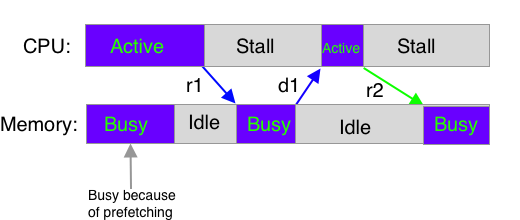
\includegraphics[width=9cm]{pictures/fig3.7}
	\caption{Hardware prefetching}
	\label{fig3.7}  %Reihenfolge ist wichtig! Immer erst \caption{} dann \label{}
\end{figure}

\subsection{Time Interval Analysis}

\begin{table} %[htbp] %hier können noch Positionierungswünsche angegeben werden
	\centering      % Alles weitere zentrieren
	\begin{tabular}{|c|c|} %Alle Spalten zentrieren, ansonsten 'r' oder 'l'
		\hline
		\textbf{Variable} & \textbf{Description}  \\
		\hline
		$T^{active}_{cpu}$               &total time when CPU is active                  \\
		\hline
		$T^{stall}_{cpu}$,	              & total time when CPU is idle              \\
		\hline
		$T^{busy}_{mem}$			& total time when memory is busy\\
		\hline				
		$T^{idle}_{mem}$				& total time when memory is idle\\
		\hline
		$fc$									& core frequency\\
		\hline
		$fuc$								& uncore frequency\\
		\hline
		$CORE\_STEP\_FREQ$  & core step frequency that changed every sampling interval\\
		\hline
		$UNCORE\_STEP\_FREQ$ & uncore step frequency that changed every sampling interval\\
		
		\hline
	\end{tabular}
	\caption{Variables used in this method}
	%\label{tab:vergleich}  %Reihenfolge ist wichtig! Immer erst \caption{} dann \label{}
\end{table}

In many situations the memory latency cannot be eliminated completely. If the Roofline model is directly applied, the total execution time that is calculated in Equation 3.1 will no longer be accurate since the data transfer and computation are not fully overlapped. Therefore, it is important to derive the transfer delay, which is a part of memory latency that cannot be hidden.  This subsection introduces the \textit{time interval analysis},  a method that determines the transfer delay. Table 3.1 describes the variables used in this method.




\subsubsection{Finding the Transfer Delay}

To find the transfer delay, the activities of both processor and memory are observed simultaneously in a time interval. Figures 3.6 and 3.7 represent the situations that the transfer delay is present. Figures 3. 8 and 3.9 show the situations that do not contain transfer delay. The following subsections discuss both situations in detail.

\textbf{With Transfer Delay}
\begin{figure} [h] %hier können noch Positionierungswünsche angegeben werden
	\centering   % Alles weitere zentrieren
	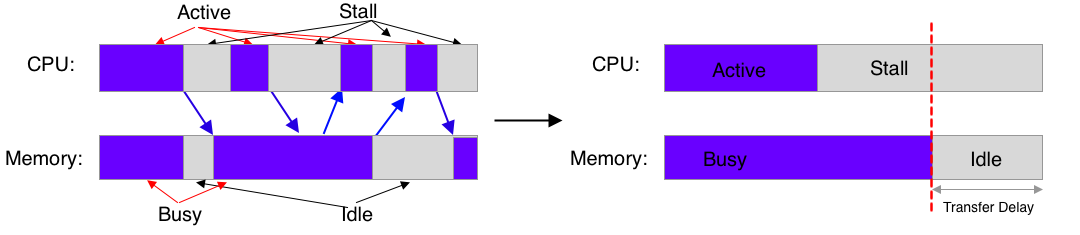
\includegraphics[width=16cm]{pictures/fig3.10}
	\caption{Real time activities vs. summarised activities of memory dominated application with transfer delay}
	\label{fig3.10}  %Reihenfolge ist wichtig! Immer erst \caption{} dann \label{}
\end{figure}
\begin{figure} [h] %hier können noch Positionierungswünsche angegeben werden
	\centering   % Alles weitere zentrieren
	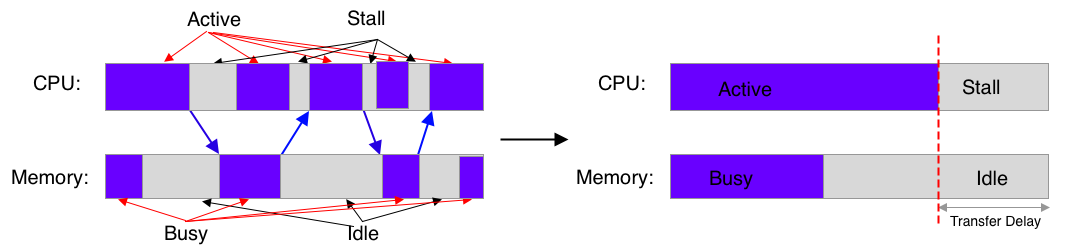
\includegraphics[width=16cm]{pictures/fig3.11}
	\caption{Real time activities vs. summarised activities of computation dominated application with transfer delay}
	\label{fig3.11}  %Reihenfolge ist wichtig! Immer erst \caption{} dann \label{}
\end{figure}

The performance is bound to transfer delay when neither the processor is $100\%$ occupied nor the memory is $100\%$ busy in the time interval. Figure 3.6 and Figure 3.7 show such situations. The figures on the left side of Figure 3.6 and Figure 3.7 illustrate the activities of the processor and memory in real-time. The processor is active for fetching, decoding, and executing instructions. The processor stalls after sending a memory request until the data is transferred to it. The arrows from the CPU to memory are memory requests and the arrows from the memory to the CPU are data transfers. 

In reality, it is hard to measure when exactly the processor is active or stalling. As a result, the right side of Figure 3.6 and Figure 3.7 illustrates the summarised activities. They measure both the active and stalling time of the processor in total and show the proportion of active and stalling time in the figure. Similarly, the total time when the memory is busy and the total time when it is idling are also measured. In this way, it is easier to both measure the data and to exhibit the results. 

The time that the CPU stalls can be derived from the hardware counters with Linux perf. The CPU's active time can be calculated by the time interval minus the CPU's stalling time. The time when memory is busy is calculated via
\begin{equation}
T^{busy}_{mem} = memVolum/Full_{BW}
\end{equation}, where the $memVolum$ is the total amount of data transfer that happens in the time interval and $Full_{BW}$ is the memory bandwidth under the current uncore frequency. The rest of the time interval for memory is idle. 


\newtheorem*{theorem*}{Theorem}
\begin{theorem*}
The transfer delay is $min\{T^{stall}_{cpu}, T^{idle}_{mem}\}$
\end{theorem*}


The transfer delay consists of the time of the memory requests and data transfer. It happens in the synchronisation of the CPU and memory. During the synchronisation, the CPU is not processing any tasks and the memory is not reading or writing any data. Therefore, the transfer delay can be characterised as the time when the memory is idle and the CPU stalls simultaneously. In Figure 3.6, the transfer delay approximates to $T^{idle}_{mem}$ while in Figure 3.7 to $T^{stall}_{cpu}$. Combining two situations, the transfer delay approximates to $min\{T^{stall}_{cpu}, T^{idle}_{mem}\}$.



\textbf{Without Transfer Delay}

\begin{figure} [h] %hier können noch Positionierungswünsche angegeben werden
	\centering   % Alles weitere zentrieren
	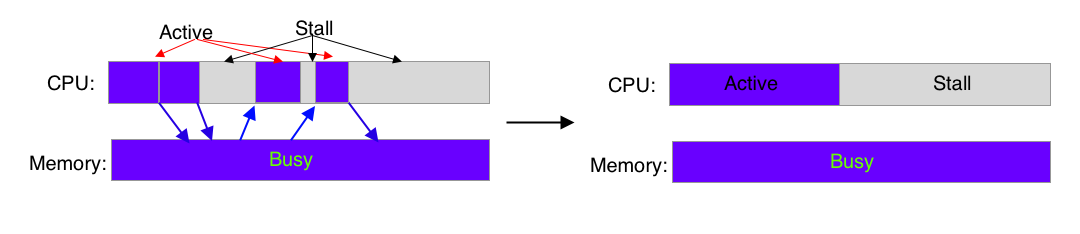
\includegraphics[width=16cm]{pictures/fig3.8}
	\caption{Real time activities vs. summarised activities of memory bound application}
	\label{fig3.8}  %Reihenfolge ist wichtig! Immer erst \caption{} dann \label{}
\end{figure}
\begin{figure} [h] %hier können noch Positionierungswünsche angegeben werden
	\centering   % Alles weitere zentrieren
	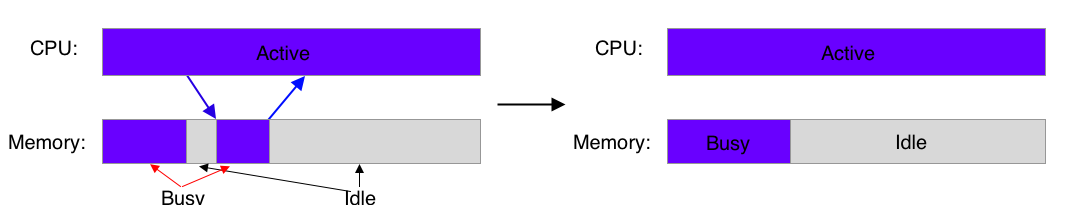
\includegraphics[width=16cm]{pictures/fig3.9}
	\caption{Real time activities vs. summarised activities of compute bound application}
	\label{fig3.9}  %Reihenfolge ist wichtig! Immer erst \caption{} dann \label{}
\end{figure}
Similar to Figures 3.6 and 3.7, Figures 3.8 and 3.9 present the real-time activities on the left and the summarised activity's time on the right. Neither of the situations contains a time slot where the memory is idle and the CPU stalls simultaneously. According to Theorem, the transfer delay approximates to $0$. The Roofline model can be applied here to determine whether it is compute-bound or memory-bound.




\chapter{Implementation}

The extended Roofline method is implemented on a Haswell node which has one Intel (R) Xeon (R) processor E5 v3 @ 2.3GHz. The processor has 18 cores. The node has 32 GB of memory.
\section{Tools: PERF and LIBMSR}
The extended Roofline method is implemented as a library via the sampling method. For every sampling interval, the function $start\_collection()$ is called to collect all the necessary hardware events. This function is integrated with Perf and Libmsr.  

Perf is a powerful tool to measure the CPU activities via accessing the performance counters. The function $perf\_event\_open()$ is used to set up performance monitoring for core events. It generates a file descriptor corresponding to a hardware event that needs to be monitored \cite{24}. Six events namely instructions, CPU cycles, reference cycles, stall cycles for L2, stall cycles for LLC and stall cycles in total are measured during each sampling interval. The file descriptors of those events are grouped together which allows events to be monitored simultaneously.  

Perf is a good tool to measure the core events, however, it lacks of uncore supports. As a result, Libmsr \cite{25} is integrated into the library to measure the uncore events. Libmsr provides an interface that allows programmers to access the MSR directly. The uncore events include the read and write volumes of DRAM and LLC and the energy consumption of PKG and DRAM. 

\section{The Extended Roofline Method}

\begin{figure} [h] %hier können noch Positionierungswünsche angegeben werden
	\centering   % Alles weitere zentrieren
	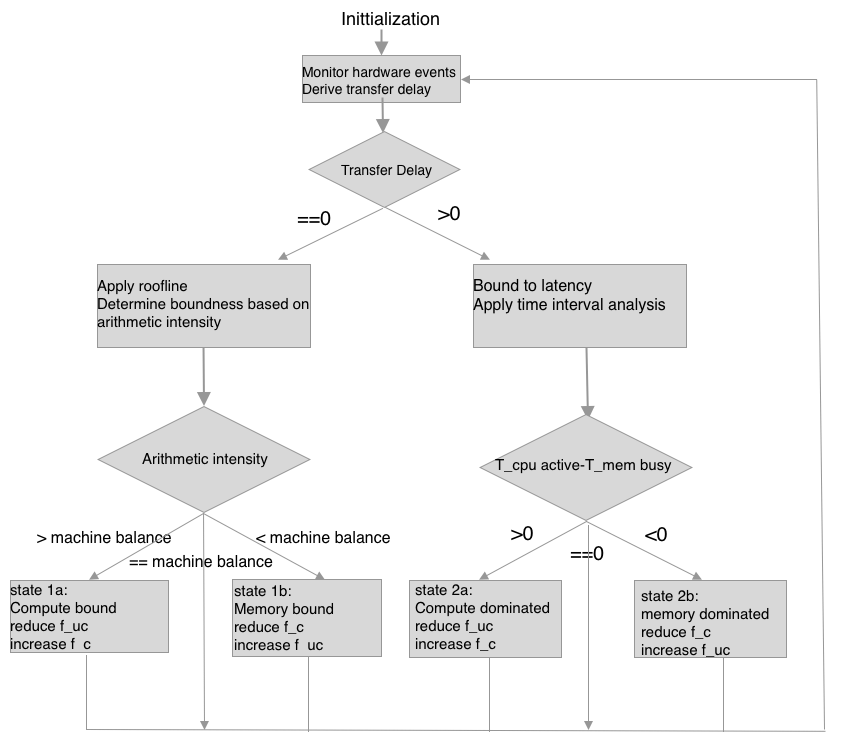
\includegraphics[width=12cm]{pictures/TIA}
	\caption{Combining the Roofline model with time interval analysis}
	%\label{fig3.7}  %Reihenfolge ist wichtig! Immer erst \caption{} dann \label{}
\end{figure}


Figure 4.1 shows the control logic of the extended Roofline method The first step is to initialise the core and uncore to their maximal frequency, $f_{c} $ = 2.8 GHz and $f_{uc} $ = 3.0 GHz. Then the hardware events are measured for each sampling interval. The sampling interval is set to 300 ms. 300 ms has minimum overhead comparing to other shorter intervals. Intervals longer than 300 ms may not detect the execution patterns correctly, e.g. it may not detect the change from memory-bound to compute-bound.
After collecting the hardware events, the function $calc\_roof()$ is called. This function first calculates the frequency of the core and uncore in Hertz, the CPU active and stall time in seconds, the busy and idle time of both DRAM and LLC in seconds and the PKG and DRAM power consumption in Watts. Then it executes the time interval analysis introduced in Section 3.3 and derives the transfer delay from the minimum of CPU stall time and memory idle time. 

If the transfer delay equals zero, the Roofline model is applied. Instead of using the FLOP/s to measure the kernel's performance in the Roofline model described in Chapter 3, the Instruction per second (IPS) is used. The reason is that not all applications perform floating-point operations only. The FLOP/s is not suitable for some applications that perform both integer operations and floating-point operations. As a result, the operational intensities of both LLC and DRAM are calculated by
\begin{equation}
operational\ intensity = \frac{instructions}{total\ data\ volume}
\end{equation}
The machine balance used in implementation is calculated as the ratio of the maximal instruction per second for the current time interval to the maximal memory bandwidth under the current uncore frequency. 
\begin{equation}
machine\ balance = \frac{maxIPS}{Full_{BW}}
\end{equation}
It is introduced in Chapter 3 that different applications have \textit{different} machine balances. The machine balance is calculated this way to guarantee it is the minimal intensity needed to reach the peak performance exclusively for the \textit{current} application in the time interval. By comparing the Equation (4.1) and (4.2), it ensures that no matter the application utilises FMA, SIMD and other ILP or not, the program always determines the correct performance bound. If the Equation (4.1) < Equation (4.2), the application is in state 1a which is compute-bound. If the Equation (4.1) > Equation (4.2), the application is in state 1b which is memory-bound. Otherwise, it is balanced.


When the transfer delay is greater than zero, the Roofline model is no longer suitable due to its inaccuracy. In this paper, this situation is defined as \textit{transfer delay bound}. The method continues to applying the time interval analysis to compare the CPU active time and memory busy time. If $T^{active}_{cpu}$ is greater than $T^{busy}_{mem}$, the system enters state 2a which is transfer delay bound dominated with computation. On the contrary, if $T^{active}_{cpu}$ is smaller than $T^{busy}_{mem}$, the system enters state 2b which is transfer delay bound dominated with memory.



\subsubsection{Side effects of frequency scaling on latency}

\begin{figure} [h] %hier können noch Positionierungswünsche angegeben werden
	\centering   % Alles weitere zentrieren
	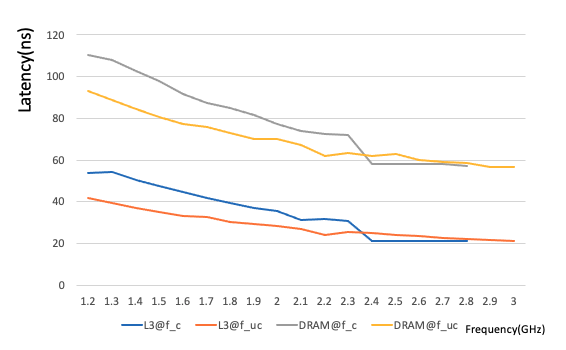
\includegraphics[width=15cm]{pictures/latency}
	\caption{L3 cache and DRAM latency change with respect to core/uncore frequency}
	%\label{fig3.9}  %Reihenfolge ist wichtig! Immer erst \caption{} dann \label{}
\end{figure}

As the clock frequencies are modified, the memory latency also changes. In the implementation, the transfer delay approximates to the latency. Figure 3.11 presents the change of the L3 cache and DRAM latency measured by the \textit{tinybench} \cite{38}. The core frequency is modified from 1.2 GHz to 2.8 GHz in steps of 0.1 GHz under the circumstance that the uncore frequency remains maximum. The uncore frequency are modified from 1.2 GHz to 3.0 GHz in steps of 0.1 GHz while keeping the core frequency at 2.8 GHz. The latency of DRAM and L3 cache decrease significantly with the increase of the core and uncore frequency. The latency of L3 decreases slower than DRAM with the increase of the core and uncore frequency. 

%The transfer delay is an essential part of the memory latency. Therefore, as the clock frequency increases, the transfer delay also increases.

\subsubsection{Modifying the CPU Clock Frequency}


%In this case, the uncore frequency is set to maximum and the core frequency is reduced by CORE\_STEP\_FREQ GHz, which is a global value that represents how much frequency will be changed in one tuning operation. Now I have to make sure that I did not over tune the core frequency. As I reduce the core frequency, the memory requests that the processor sends to the memory will be smaller. As a result, the memory idle time will be greater and we have a new time interval $T_{new}$ which is the time when memory is busy plus the new memory idle time. To determine whether the new time interval is too large that indicates an performance degradation, we simply compare $T_{new}$ with the execution time $T_{atMax}$ where the core frequency is maximum. If
%\begin{equation}
% T_{new} > T_{atMax} * (1 + ROOF\_THRESHOLD), 
%\end{equation}
%it shows that the new time interval exceeds the execution time when the core is maximum which indicates we have over reduced the core frequency. It heavily downgrades the performance, as a result the core frequency will be increased by CORE\_STEP\_FREQ. The ROOF\_THRESHOLD is a predefined threshold value.
%
The tuning of the CPU clock frequency contains two situations. One of them is the tuning does not concern any power cap. The other one is when there exists a power cap. The goal is to reduce the power consumption and in the meantime try not to downgrade the performance too much. 



\textbf{Without power cap}

For compute-bound state 1a, the $f_{uc}$ is reduced by \textit{UNCORE\_STEP\_FREQ} and the $f_c$ is set to maximum. For memory-bound state 1b, the $f_c$ is reduced by $CORE\_STEP\_FREQ$ and the $f_{uc}$ is set to maximum. For transfer delay bound with compute domination state 2a, the $f_{c}$ will be set to the maximum while the $f_{uc}$ is reduced by $UNCORE\_STEP\_FREQ$. As the uncore frequency decreases, the transfer delay increases respectively. Therefore, the time interval is increased. The new time interval is derived as $T_{new}$. A threshold needs to be defined to ensure the new time interval is not too large. Otherwise, it will cause performance downgrading. The threshold is set to $T_{atMax}* (1 + ROOF\_THRESHOLD)$. $T_{atMax}$ is the execution time where the uncore frequency is maximum. $ROOF\_THRESHOLD$ is a predefined value for precision tolerance. If
\begin{equation}
 T_{new} > T_{atMax} * (1 + ROOF\_THRESHOLD), 
\end{equation}
the core frequency will be re-added by $CORE\_STEP\_FREQ$.

For transfer delay bound with memory domination state 2b, the uncore frequency will be set to the maximum while the core frequency is reduced one step lower. The new time interval is calculated and compared with $T_{atMax}* (1 + ROOF\_THRESHOLD)$. The $T_{atMax}$ in this state is the execution time wherer the core frequency is maximum. If Equation 4.3 holds, it indicates that the new time interval exceeds the limit. Therefore, the core frequency is increased by $CORE\_STEP\_FREQ$.

\textbf{With power cap}

Under the circumstance that the power consumption has an upper limit, the tuning strategy should be reconsidered. For the state 2a, the $f_{uc}$ is decreased by $UNCORE\_STEP\_FREQ$ first. Since the uncore frequency is decreased, the system releases a small amount of power budget which can be used to increase the $f_c$. As the core and uncore frequency are modified simultaneously, the $T^{active}_{cpu}$, $T^{busy}_{mem}$, transfer delay, and the time interval also change. It is important to ensure the frequencies are not over-tuned. To do that, the algorithm compares $T^{active}_{cpu}$ with $T^{busy}_{mem}$ The CPU active time should be greater than the memory busy time. Otherwise, it suggests the application that is supposed to be compute dominated is changed to be memory dominated. If an over-tune is detected, the $f_{uc}$ is increased by $CORE\_STEP\_FREQ$. For state 2b, the tuning will be vice versa.
%Figure 3.10 shows the other case where it is compute bound. Since the processor dominates in the time interval, we have to divide it into two parts, one is the time that is bound to computation, and the other is bound to transfer delay. The transfer delay in this case is equal to the time when the processor stalls. The core frequency will be set to maximum while the uncore frequency is reduced one step lower. As I reduce the uncore frequency, the memory controllers that are responsible for data transfer between the memory and the processor will operate slower and make processor spend more time waiting for the data. Therefore the processor's stalling time will increase and we have to recalculate the time interval $T_{new}$ which is the time when processor is active plus the new processor's stalling time. Then I simply compare $T_{new}$ with the the execution time $T_{atMax}$ where the uncore frequency is maximum. If equation 3.3 holds, it shows that the new time interval exceeds the limit and I have to increase the uncore frequency one step higher.
%


\chapter{Experiments and Evaluations}

The experiments are divided into two groups. One of which compares the extended Roofline method on memory-bound and LLC cache-bound applications using the STREAM benchmark. The STREAM benchmark is used to showcase the boundary cases. The other one uses NAS parallel benchmarks \cite{23} to compare the results on applications that are compute-bound, memory-bound and LLC cache bound. The NAS parallel benchmark suite ensures that the evaluation on the extended Roofline method covers as many types of applications as possible. 

\section{Evaluation with STREAM benchmark}
STREAM benchmark is used to evaluate the extended roofline model on memory-bound program. The problem size in STREAM source code is modified to obtain two kinds of output files namely $stream_{DRAM}$ and $stream_{L3}$. In $stream_{DRAM}$, the total memory required is much greater than the size of the L3 cache so that it can correctly measure the DRAM bandwidth. In $stream_{L3}$, the problem size is reduced so that the total memory required is less than the L3 cache but greater than the L2 cache. In this way, the STREAM is able to measure the L3 cache bandwidth correctly. The $stream_{L3}$ can be therefore characterised as an LLC-bound benchmark.

The stream benchmark and the extended Roofline method were running simultaneously on two terminal windows. The clock frequencies, PKG power, DRAM power and slowdown are recorded. Each experiment was repeated 3 times and the average value is presented. 

\begin{figure} [h] %hier können noch Positionierungswünsche angegeben werden
	\centering   % Alles weitere zentrieren
	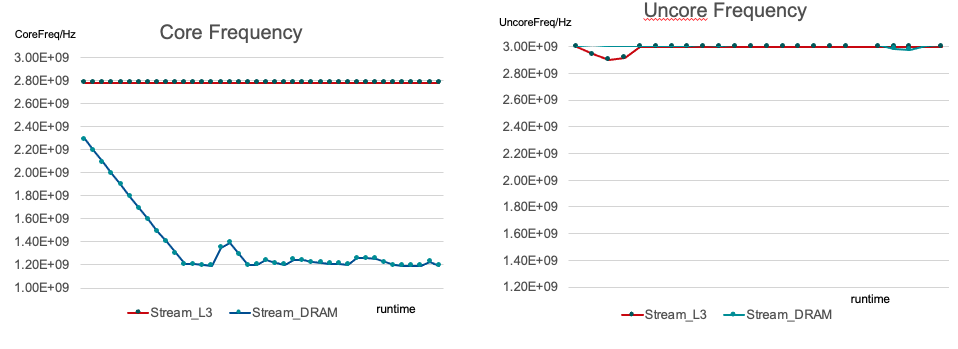
\includegraphics[width=17cm]{pictures/cuc}
	\caption{Core vs. uncore frequency of STREAM}
	%\label{fig1}  %Reihenfolge ist wichtig! Immer erst \caption{} dann \label{}
\end{figure}

Figure 5.1 illustrates the core and uncore frequency of both $stream_{DRAM}$ and $stream_{L3}$ during runtime. The x-axis shows the runtime while the y-axis represents the frequency. The figure on the left compares the core frequency of both stream programs. The core frequency of $stream_{DRAM}$ decreases linearly first and remains minimal afterwards. The reason is that the $stream_{DRAM}$ is memory intensive and it heavily utilises the memory controllers located in the uncore area. The processor core wastes large amounts of cycles stalled for memory. The extended Roofline method detects such situations and lowers the core frequency respectively. The frequency of  $stream_{L3}$ remains maximal since the extended Roofline method suggests the arithmetic intensity approximates to the machine balance. $Stream_{L3}$ is LLC intensive and most data transfers happened between L2 and LLC. The processor can access the data faster and spend less time stalling (only 1\% of the time interval). Therefore, the core frequency should not be decreased. The figure on the right shows the uncore frequency remains maximal for both stream programs because both of them utilise the uncore heavily.

	
Table 5.1 shows the PKG power in Watts, PKG energy in Joules and completion time in seconds for default setting where the core and uncore frequency is maximum. The metrics are measured with LIKWID. Figure 5.2 shows the PKG power saving and energy saving in Watts and slowdown compared to the default setting. The x-axis shows different performance groups and the y-axis represents the results that are normalised with respect to the default.

\begin{table} [h] %hier können noch Positionierungswünsche angegeben werden
	\centering      % Alles weitere zentrieren
	\begin{tabular}{|c|c|c|} %Alle Spalten zentrieren, ansonsten 'r' oder 'l'
		\hline
		\textbf{Metric} & \textbf{stream\_dram} &\textbf{stream\_L3}  \\
		\hline
		Completion time(s)              & 22 &11.5       \\
		\hline
		PKG power(W)	              &  140& 119       \\
		\hline
		PKG energy(J)		 &   2990 &   1683  \\
		
		\hline
	\end{tabular}
	\caption{Performance metrics for Stream DRAM and L3 by default when $f_c$ = 2.8 GHz and $f_{uc}$ = 3.0 GHz}
	%\label{tab:vergleich}  %Reihenfolge ist wichtig! Immer erst \caption{} dann \label{}
\end{table}

\textit{Observation 1: The extended Roofline method saves up to 40\% PKG power and energy for STREAM benchmark}

The extended Roofline method saves 38\% PKG power on $stream_{DRAM}$ compared to the default. This is because it detects the application is memory-bound and reduces the core frequency. The energy consumption also reduces due to the drop of PKG power because the energy equals the power multiplied by time. On the other hand, the extended Roofline method has minor effects on the $stream_{L3}$. The reason is that $stream_{L3}$ is balanced for computation and data communication.

\textit{Observation 2: The extended Roofline method has little impact on performance downgrading}

The job completion time is used to represent the performance downgrading. as observed from Figure 5.2, the job completion time increases by 3.2\% for $stream_{DRAM}$. This indicates the extended Roofline method has little impact on performance downgrading for memory streaming which is totally acceptable. For compute-memory-balanced programs, the performance downgrading can be ignored since the slowdown is only 0.4\%.


	
\begin{figure} [h] %hier können noch Positionierungswünsche angegeben werden
	\centering   % Alles weitere zentrieren
	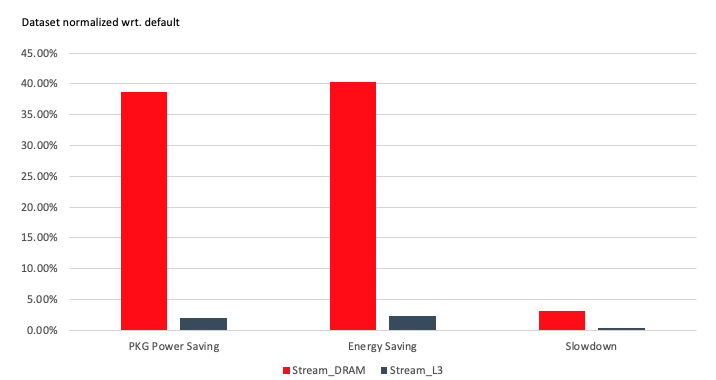
\includegraphics[width=17cm]{pictures/Stream}
	\caption{Evaluation on STREAM}
	%\label{fig1}  %Reihenfolge ist wichtig! Immer erst \caption{} dann \label{}
\end{figure}

\section{Evaluation with NAS Parallel Benchmarks}

The second group of experiments was carried out using Embarrassingly Parallel (EP),  Conjugate Gradient (CG),  Block Tri-diagonal solver (BT), Multi-Grid (MG), Fourier Transform (FT) and Scalar Penta-diagonal solver (SP) from the NAS parallel benchmark suite \cite{23}. The EP is compute-intensive, the CG is memory-bound and known for its irregular memory access and communication, MG and FT are memory-intensive programs \cite{23}. SP is LLC intensive and BT is LLC intensive with constantly changing DRAM usage \cite{21}. The openMP version of these benchmarks is used and the input sizes B and C are used in experiments.

The core and uncore frequency is maximal by default. The PKG power in Watts, PKG energy in Joules and the completion time in seconds are measured with LIKWID for the default setting. Each of the benchmarks and the extended Roofline method are executed simultaneously in two terminal windows and the performance metrics are recorded by the extended Roofline method. Each experiment is repeated three times and the average values of the results are calculated. 

Figure 5.3 presents the PKG power and energy saving and slowdown compared to the default setting. The x-axis shows the groups of those performance metrics. Each of the groups contains six columns representing EP, CG, BT, MG, FT and SP from left to right. The y-axis presents the value normalized with respect to the default measurements.

\begin{figure} [h] %hier können noch Positionierungswünsche angegeben werden
	\centering   % Alles weitere zentrieren
	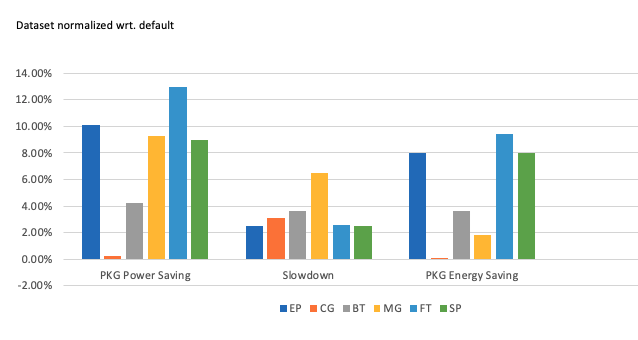
\includegraphics[width=17cm]{pictures/NPB}
	\caption{PKG power and energy saving and slowdown wrt. default}
	%\label{fig1}  %Reihenfolge ist wichtig! Immer erst \caption{} dann \label{}
\end{figure}


\textbf{EP}

The extended Roofline method achieves 10\% of PKG power saving and 8\% of PKG energy saving with a slight slowdown of 2.2\%. The program correctly detects the compute-intensive characteristic of EP. Figure 5.4 shows the activities of the CPU and memory detected by the time interval analysis. The processor occupied 83\% of the time interval while the memory is 99.8\% idle. In this case, the program sees the application as compute-bound and reduces the uncore frequency. The slowdown caused by the overhead of the program is only 2.2\% which is acceptable compared to the percentage of the power and energy saving. The slowdown on EP is one of the lowest among all other benchmarks. Therefore, the extended Roofline method performs well on compute-intensive benchmarks.

\begin{figure} [h] %hier können noch Positionierungswünsche angegeben werden
	\centering   % Alles weitere zentrieren
	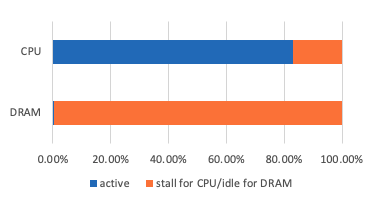
\includegraphics[width=9cm]{pictures/timeforep}
	\caption{Activities of CPU and DRAM in a sampling interval on EP}
	%\label{fig1}  %Reihenfolge ist wichtig! Immer erst \caption{} dann \label{}
\end{figure}

\textbf{CG}

The extended Roofline method has little impact on the power or energy saving on CG. It detects that CG is bound to transfer delay with memory domination. However, the core frequency is not reduced because it will lead to severe performance downgrading. As a result, the frequency should remain default for CG.  The extended Roofline method brings 3.1\% slowdown to the application because of the overhead of accessing hardware counters and interrupt for each sampling interval.

\textbf{BT and SP}

Figure 5.5 illustrates the measured core and uncore frequency. The core and uncore frequency keep being modified between 2.4 to 2.6 GHz for BT during runtime. It is because the DRAM access of BT varies during runtime. BT's execution patterns vary from memory-dominated to compute-dominated. When BT is memory-intensive, it utilises uncore heavily. The uncore frequency is higher and the core frequency is lower. When BT transits to compute-intensive, the uncore frequency becomes lower while the core frequency becomes higher. The changing of the core and uncore frequency leads to  4.2\% PKG power saving and 3.8\% of PKG energy saving. The slowdown is 3.7\% caused by standard overhead.

The extended Roofline method performs well on SP since it achieves more than 8\% of PKG power and energy saving. The slowdown is only 2.2\%. 


\begin{figure} [h] %hier können noch Positionierungswünsche angegeben werden
	\centering   % Alles weitere zentrieren
	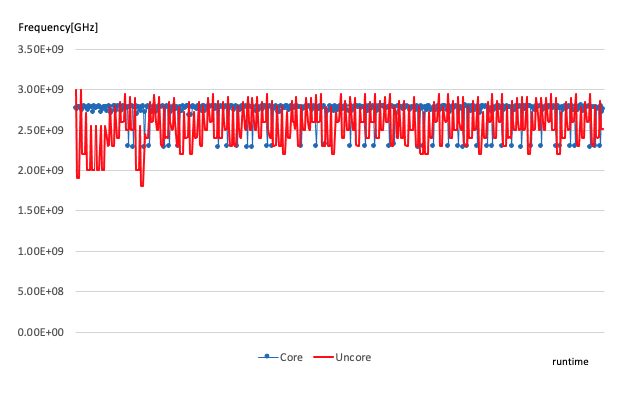
\includegraphics[width=12cm]{pictures/bt_fcuc}
	\caption{Frequency of BT from NPB}
	%\label{fig1}  %Reihenfolge ist wichtig! Immer erst \caption{} dann \label{}
\end{figure}

\textbf{MG and FT}

The core frequency is reduced and the uncore frequency remains maximal for these two memory-intensive benchmarks. The extended Roofline method achieves up to 13\% of PKG power saving and 9.4\% of energy saving. The slowdown on FT is insignificant while on MG is greater. \\

In conclusion, the extended Roofline method achieves up to 13\% PKG power saving and 9.4\% PKG energy saving with the slowdown in the worst case 6.5\%.

\subsubsection{Evaluation under the power cap}

While the frequency tuning strategy of the situations under a power cap is different from those that do not have a power cap. The evaluation of the programs under the power cap is also needed. In this experiment, RAPL is used to set the power cap of the processor. The power cap is set to the minimum which is 69W to compare the extended Roofline method with the default setting. Figure 5.6 shows the total energy saving (PKG + DRAM energy) and the speedup with respect to the default on the NAS parallel benchmark suite under the power cap. The x-axis shows the groups of the performance metrics. The y-axis presents the data normalized with respect to default. The extended Roofline method achieves up to 6.2\% speedup over default. It reveals that the extended Roofline method outperforms the default setting under strict power constraints. Spending less time completing the tasks leads to less energy consumption. During the experiment, the extended Roofline method keeps the power consumption lower than the default. Lower power consumption and shorter execution time lead to 8.9\% energy saving in the best case across all benchmarks

\begin{figure} [h] %hier können noch Positionierungswünsche angegeben werden
	\centering   % Alles weitere zentrieren
	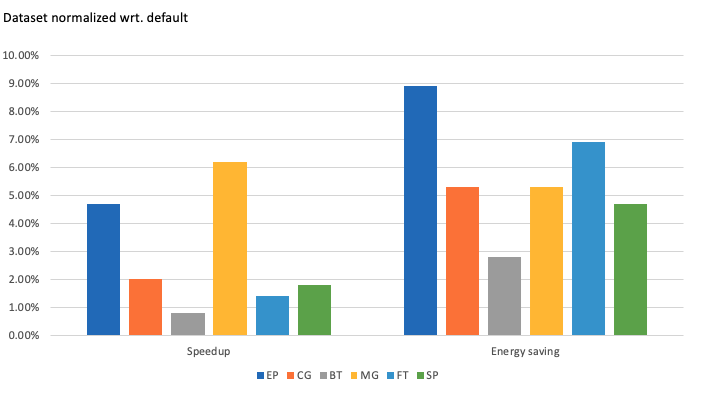
\includegraphics[width=15cm]{pictures/cap}
	\caption{Total energy saving and speedup wrt. default under power cap}
	%\label{fig1}  %Reihenfolge ist wichtig! Immer erst \caption{} dann \label{}
\end{figure}






\chapter{Related Work}

\section{Previous researches on the Roofline model}
Ofenbeck et al.  \cite{28} studied how to apply the Roofline model on Intel platforms. They provided an approach to measure the necessary data of a running program and to produce the Roofline plot based on the data. Ilic et al. \cite{27} proposed the cache-aware Roofline model which is able to model the performance on multiple levels of caches. Hill et al. \cite{29} proposed the Gables model which refines the Roofline model in a way that it can be applied on system-on-chips (SoC). SoC is a widely used architecture on modern smartphones. It integrates the CPU, memory, GPU and other necessary components in a single microchip \cite{30}. Gables is able to model the performance bound of different components of SoC which guides the developer to optimise the performance. Kim et al. \cite{31} used the Roofline model to analyse and optimise the performance of the Finite-Difference Time-Domain (FDTD) on GPU. FDTD is a numerical technique to simulate the electromagnetic field \cite{32}. They pointed out that memory access optimisations are most important for GPU.  Ding et al. \cite{33} proposed the instruction Roofline model for GPUs. They used the instruction-oriented approach to characterise the performance which is an inspiration of the implementation in this work. Cabezas et al. \cite{35} extended the Roofline model with multiple hardware-related bottlenecks such as throughput, latency, OoOE buffers and capacity information for a multi-level cache hierarchy. They integrated those bottlenecks into one Roofline plot. Sato et al. \cite{36} model the performance of the vector processors with the vector cache using the Roofline model. They proposed optimisation strategies that reduce energy consumption up to 70\%.


The studies mentioned above apply the Roofline model to model and optimise the performance. This paper aims to dynamically modify the clock frequency to achieve power saving based on the Roofline model. This work differs from them by combining the Roofline model with time interval analysis which characterises the performance bound under memory access latency. 

\section{Previous researches on power management}
Gholkar et al. \cite{21} proposed the uncore power Scavenger (UPScavanger), a runtime system that dynamically changes the uncore frequency to achieve power and energy saving. It is able to detect the execution patterns (memory-bound or compute-bound) of an application based on the changing of the DRAM power and IPC. They compared the UPScavenger with Intel's default uncore power setting and showed that the UPScavenger achieves considerable power saving. They also compared it with Intel's RALP under the same power cap and showed that it speeds up the completion of a task. This paper differs from it by identifying the execution patterns based on the Roofline model and time interval analysis. Besides, work modifies both core and uncore frequency to achieve power saving.
Sundriyal et al. \cite{34} explored how the uncore frequency affects memory latency and bandwidth. They also compared the energy saving of the UFS and DVFS on quantum chemistry application GAMESS. They stated that combining the UFS and DVFS achieves significant energy saving on GAMESS. In this paper, the effect of both core and uncore frequency on memory latency is explored.
Gupta et al. \cite{37} observed the uncore power consumption in a heterogeneous computing system that contains both high and low power cores, which is a typical processor architecture for modern smartphones. They claimed that heterogeneous core architectures have huge advantages over homogeneous for the client device in terms of energy efficiency. They concluded that the uncore component is potentially a huge contribution to power saving.



\chapter{Conclusion}

In this work, I studied the architecture of the microprocessor and explored the impact of uncore frequency on PKG power, DRAM power and bandwidth. I explored how to use the Roofline model to characterise the performance bottleneck on  processors. The extended Roofline model is developed. It combines the traditional Roofline with time interval analysis to detect the transfer delay and optimizes the performance by dynamically modifying the core and uncore frequencies. In situations that do not have a power cap, it saves up to 13\% PKG power and 9.4\% PKG energy. The slowdown varies from 2\% to 6.5\% compared to the default. In situations that have strict power constraints, it saves up to 8.9\% energy and achieves in best case 6.2\% speedup compared to the default.

The improvement on the overhead reduction is a possible future work. This work implements the extended Roofline via the time sampling method. Other sampling approaches such as sampling by instruction is also a possible future study. 



%%%%%%%%%%%%%%%%%%%%%%%%%%%%%%%%%%%%%%%%%%%%%%%%%%%%%
% Der Anhang (andere Sektionsnummerierung)
%%%%%%%%%%%%%%%%%%%%%%%%%%%%%%%%%%%%%%%%%%%%%%%%%%%%%
\appendix
% Hier werden die Anhänge eingebunden
% TODO : weitere Kapitel in my_appendices.tex eintragen
% Hier die Kapitel des Anhangs einf�gen
\include{appendix_background}




%
\bibliography{gesammelte_werke} %Literaturverzeichnis
\bibliographystyle{abbrv}       %Stil des Literaturverzeichnisses (en)
%\bibliographystyle{abbrvdin}       %Stil des Literaturverzeichnisses (de)

% evtl. Abkuerzungsverzeichnis (z.B. Paket nomenclature)

\printindex                     % Wenn ein Index erstellt werden soll, muss
                                %  diese Zeile aktiviert werden
                                %  Zusaetzlich oben das Paket einbinden und \makeindex

\end{document}



